\vfill
\section{Development and training}

The original Model design and training was done in Python using the PyTorch deep learning library. Semantic segmentation was performed using the Deeplabv3 architecture. The segmentation model had a base architecture of a 50-layer residual net and minimized pixel-level binary crossentropy loss. The model was initialized with random weights and was trained using a stochastic gradient descent optimizer. We assessed three model architectures with variable integration of temporal convolutions (R3D, MC3 and R2+1D) and ultimately chose decomposed R2+1D spatiotemporal convolutions as the architecture with the best performance to use for EchoNet-Dynamic. In the R3D architecture, all convolutional layers considered the spatial and temporal dimensions jointly and these consisted of five convolutional blocks. The MC3 and R2+1D architectures were introduced as a middle ground between two-dimensional convolutions that considered only spatial relationships and the full three-dimensional convolutions used by R3D. The MC3 architecture replaced the convolutions in the final three blocks with two-dimensional convolutions, and the R2+1 architecture explicitly factored all of the three-dimensional convolutions into a two-dimensional spatial convolution followed by a one-dimensional temporal convolution.

We did a upgrade In the semantic segmentation model phase, we integrated the UNet++ architecture to enhance performance. We dissected the Deeplabv3 architecture from torchvision, added transformation layers to the backbone, and connected it with the UNet++ network. The output of this new network was then connected with a classifier, forming our new model. This integration aims to achieve more accurate semantic segmentation.

While we add a UNet model,the model size increased a lot. We hope it can get a much smaller size of model and also keep the model performance. So we use knowledge-distillation to achive it.  At phase one we use Deeplabv3-Resnet50 + UNet++ 5 Levels with mean to find best model as teacher,and use Resnet18 and Resnet34 as the student,using Output layer Distillation method with loss function as following:

\begin{figure}[h]
\centering
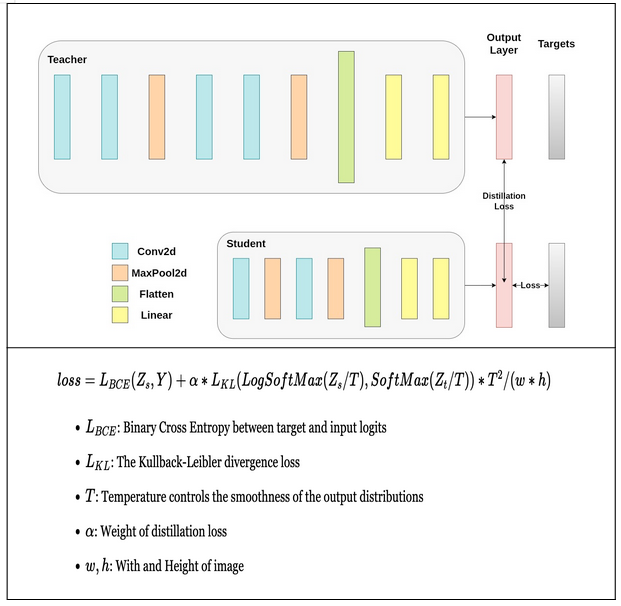
\includegraphics[width=0.5\textwidth]{dev1}
\label{dev0}
\end{figure}

For predicting ejection fraction, the models were trained to minimize the squared loss between the prediction and true ejection fraction using a stochastic gradient descent optimizer with an initial learning rate of 0.0001, momentum of 0.9 and batch size of 16 for 45 epochs. The learning rate was decayed by a factor of 0.1 every 15 epochs. For model input, video clips of 32 frames were generated by sampling every other frame (sampling period of 2) with both clip length and sampling period determined by hyperparameter search. During training, to augment the size of the dataset and increase the variation of exposed training clips, each training video clip was padded with 12 pixels on each side, and a random crop of the original frame size was taken to simulate slight translations and changes in camera location. For all models, the weights from the epoch with the lowest validation loss was selected for final testing. Model computational using one NVIDIA GeForce RTX 4070 Ti GPU.


